\section{Более общие структуры данных}

Рисунок 8.3 --- это версия рисунка 8.1, в применении к общим структурам данных $P \to \textbf{x}$. Между этими двумя рисунками нет особой концептуальной разницы, за исключением уровня обобщения. В реальном мире неизвестный вероятностный механизм $P$ порождает наблюдаемый набор данных $\textbf{x}$ в соответствии с правилом построения, указанным стрелкой «$\to$». В конкретных приложениях нам нужно более тщательно определять стрелку, наподобие того как в (8.5) для двухвыборочной задачи. Набор данных $\textbf{x}$ больше не может быть одним вектором. Он имеет форму, зависящую от структуры данных, например $\textbf{x} = (\textbf{z}, \textbf{y})$ в двухвыборочной задаче.\\
\noindent
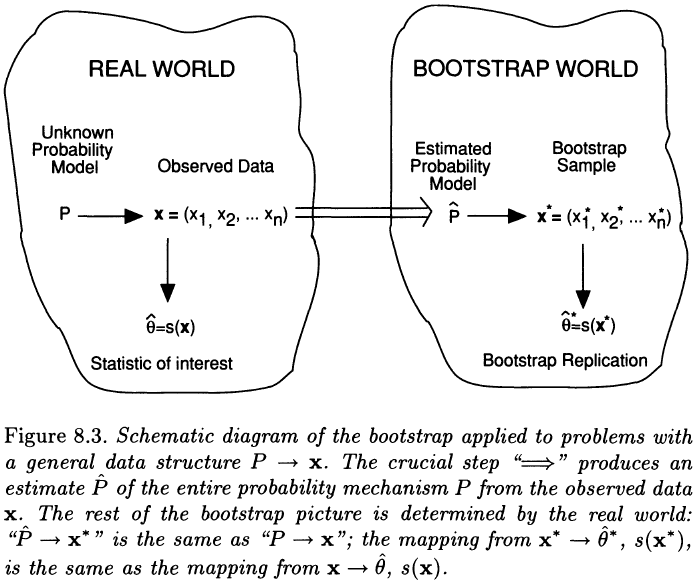
\includegraphics[width=\linewidth]{8/f83}
\newline
\noindent Наблюдая за $\textbf{x}$, мы вычисляем интересующую статистику $\hat{\theta}$ из $\textbf{x}$ в соответствии с функцией $s(\cdot)$.

Бутстреп часть на рис. 8.3 описывается аналогичными понятиями и в реальном мире: стрелка в $\hat{P} \to \textbf{x}^*$ означает то же самое, что и стрелка в $P \to \textbf{x}$. И функция, отображающая $\textbf{x}^*$ в $\hat{\theta}^*$, является той же функцией $s(\cdot)$, что и отображающая $\textbf{x}$ в $\hat{\theta}$. 

При фактическом проведении бутстреп анализа на основе рисунка 8.3 возникают две практические задачи:

(1). Нам нужно оценить весь вероятностный механизм $P$ по наблюдаемым данным $\textbf{x}$. Это шаг, обозначенный двойной стрелкой $\textbf{x} \Rightarrow \hat{P}$. Это удивительно легко сделать для большинства знакомых структур данных. Универсального рецепта нет, но в каждом отдельном случае доступны вполне обычные конкретные решения, например, $\hat{P} = (\hat{F}, \hat{G})$ для двухвыборочной задачи. Дополнительные примеры приведены в этой и следующей главах.

(2). Нам нужно смоделировать бутстреп данные из $\hat{P}$ в соответствии с подходящей структурой данных. Это шаг $\hat{P} \to \textbf{x}^*$ изображен на рисунке 8.3. Этот шаг концептуально прост, будучи таким же, как $P \to \textbf{x}$, но может потребовать некоторой осторожности при программировании, если необходима вычислительная эффективность. (Мы увидим пример данных про анализ лютенизирующего гормона ниже.) Обычно генерация бутстреп данных $\hat{P} \to \textbf{x}^*$ требует меньше времени, чем вычисление $\hat{\theta}^* = s(\textbf{x}^*)$.

\noindent
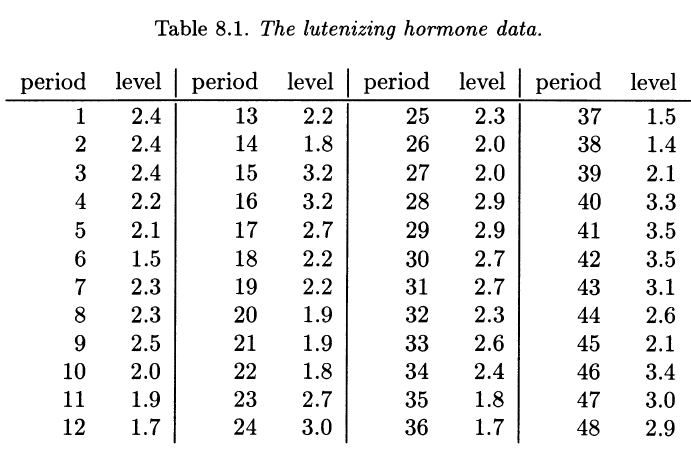
\includegraphics[width=12cm]{8/t81}\\